\section{Motivation}
\label{sec:motive}

\begin{figure}
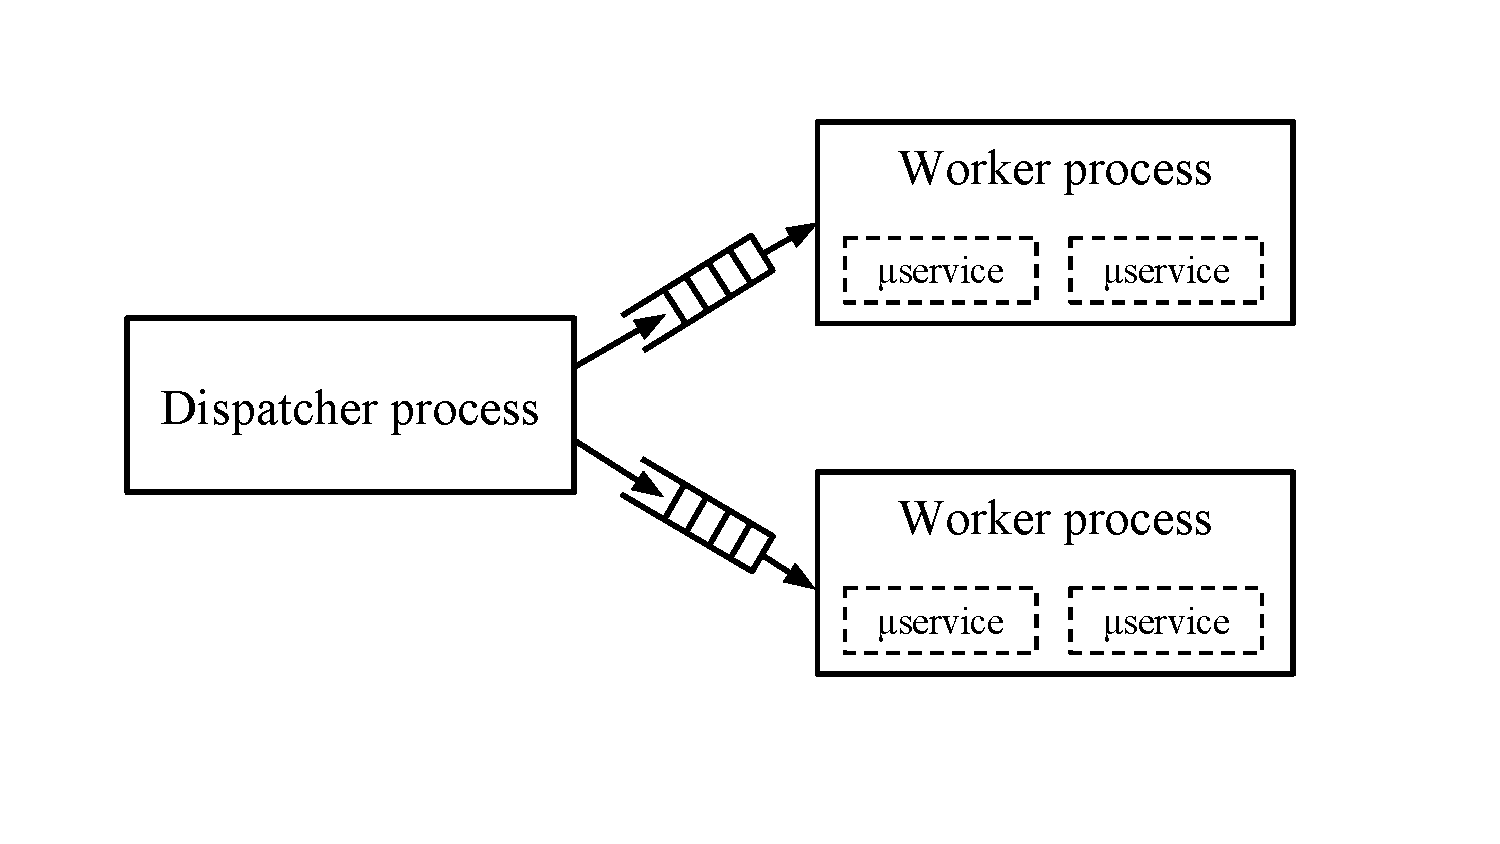
\includegraphics[width=\columnwidth]{figs/fancy_system}
\caption{Language-based isolation design.  The dispatcher process
uses shared in-memory queues to feed requests to the worker processes, each of
which runs one user-supplied microservice at a time.}
\label{fig:sysdesign}
\end{figure}

Our decision to use language-based isolation is based on two experimental
findings:  (1) Process-level isolation is too slow for
microsecond-scale user functions. (2) Commodity
CPUs support task preemption at microsecond scale.  We conducted our experiments
on a single Intel\textcopyright\@ Xeon\textcopyright\@ E5-2683 v4 server (16 cores, 2.1~GHz) running
Linux 4.13.0.\footnote{\solb{Add link to source code repo.}}

\subsection{Process-level isolation is too slow}
We use a single-machine experiment to evaluate the invocation overhead of different
isolation mechanisms: We use 14 \emph{worker} CPU cores to run microservices. Another
core runs a \emph{dispatcher} process that initiates microservice execution on the
workers.  All requests originate
from the dispatcher (which in the case of a full serverless platform would instead
forward from a cluster-level scheduler).  The dispatcher schedules up to 14
microservices at a time (i.e., one per worker core), choosing from a pool of 5,000.

To provide a comparison against contemporary system designs, we use two different
isolation mechanisms:
\begin{enumerate}
\item \textbf{Process-based isolation:} Each microservice is a separate process.
We expect this approach to exhibit lower latency than the container isolation common
in contemporary serverless deployments.
\item \textbf{Language-based isolation:} Each worker core hosts a single-threaded
\emph{worker process} that directly executes different microservices, one at a time.
In this approach, shown in Figure~\ref{fig:sysdesign}, a worker process runs a
microservice by calling its registered
function; we assume that the microservice function can be isolated from the
worker process with language-based isolation techniques that we discuss in
Section~\ref{sec:isolation}. The dispatcher schedules microservices on worker
processes by sending them
requests on a shared memory queue, which idle worker processes poll.
\end{enumerate}

\noindent
We use 5,000 copies of a microservice that simply records a timestamp:\@
latency is measured between when the dispatcher invokes a microservice
and the time that microservice records.  There are two experiment modes:

\paragraph{Warm-start requests.}
We first model a situation where all of the microservices are already resident on the
compute node.  In the case of process-based isolation, the dispatcher launches all
5,000 microservices at the beginning of the experiment, but they all block on an IPC
call; the dispatcher then invokes each microservice by waking up its process using a
UDP datagram.  In the case of language-based isolation, the microservices are
dynamic libraries preloaded into the worker processes.

\begin{table}
\begin{center}
\small
\begin{tabular}{@{}llrrc@{}}
  \multicolumn{2}{c}{\textbf{Microservices}} & \multicolumn{2}{c}{\textbf{Latency (µs)}} & \textbf{Throughput} \\
  \textbf{Resident?} & \textbf{Isolation} & Median & 99\% & \textbf{(M invoc/s)} \\
\midrule
\multirow{2}{*}{Warm-start} & Process & 8.7 & 27.3 & 0.29 \\
& Language & 1.2 & 2.0 & 5.4~~ \\
\midrule
\multirow{2}{*}{Cold-start} & Process & 2845.8 & 15976.0 & \multicolumn{1}{c}{---} \\
& Language & 38.7 & 42.2 & \multicolumn{1}{c}{---} \\
\end{tabular}
\caption{Microservice invocation performance}
\label{tab:invocperf}
\end{center}
\vspace{-12pt}
\end{table}

Table~\ref{tab:invocperf} shows the latency and throughput of the two
methods.  We find that the process-based isolation approach takes \us{9} and achieves
only 300,000 warm microservice invocations per second. In contrast, language-based
isolation achieves \us{1.2} latency (with a tail of just \us{2.0}) and over 5 million
invocations per second.

Considering that the FaRM distributed computing platform
achieved mean TATP transaction commit latencies as low as
\us{19} in 2015~\cite{Dragojevic:sosp2015}, a \us{9} delay in microservice invocation
already represents almost 50\% overhead for a microservice providing a thin API
gateway to such a backend service.  We therefore conclude that even in the average
case, process-based isolation is too slow for microsecond-scale scheduling.
Furthermore, IPC overhead limits invocation throughput.

Process-based isolation also has a higher memory footprint:\@ loading the 5,000
trivial microservices consumes 2 GiB of memory with the process-based approach, but
only 1.3 GiB with the language-based one.  However, this benefit may reduce as
microservices' code sizes increase.

\paragraph{Cold-start requests.}
Achieving ideal wakeup times is possible only when the microservices are
already resident, but the tail latency of the serverless platform depends on
those requests whose microservices must be loaded
before they can be invoked.  To assess the difference between process-based and
language-based isolation in this context, we run the experiment with the following
change:  In the former case, the dispatcher now launches a transient
microservice process for each request by \texttt{fork()/exec()}'ing.  In the latter,
the dispatcher asks a worker to load a microservice's dynamic library (and
unload it afterward).  The results in Table~\ref{tab:invocperf} reveal an
order-of-magnitude slip in the language-based approach's latency; however, this is
overshadowed by the three orders of magnitude increase for process-based
isolation.

\subsection{Intra-process preemption is fast}
In a serverless system using language-based isolation, a cluser-level scheduler would
handle routing of requests to individual worker nodes.  Since we run user-provided
microservices directly in worker processes, a rogue long-running microservice could
thwart such scheduling by unexpectedly consuming the resources of a worker that
already had numerous other requests queued.  We hypothesize that, in such situations,
it is better for tail latency to preempt the long microservice than retarget the
waiting jobs to other nodes in real time.  At our scale, this means a preemption
interval up to two orders of magnitude faster than Linux's default \ms{4} process
scheduling quantum.

Fortunately, we find that high-precision event timers (HPETs) on modern CPUs
are sufficient for this task. We measure the granularity and reliability of
these timers as follows: We install a signal handler and configure a POSIX timer to
trigger it every $T$~\textmu{}s.
Ideally, this handler would always be called exactly $T$~\textmu{}s after its last
invocation; we measure the deviation from $T$ over 256 iterations.
We find that the variance
is smaller than 0.3~\textmu{}s for $T \ge 3$~\textmu{}s. This shows that
intra-process preemption is fast and reliable enough for our needs.
